\documentclass[a4paper,11pt] {article}
\hfuzz=100pt 
%\documentclass[a4paper,article,oneside,10pt]{memoir}
\usepackage[latin1]{inputenc}
\usepackage[T1]{fontenc}
%\usepackage[lucidasmallscale, nofontinfo]{lucimatx}
%\usepackage{times}
\usepackage{graphicx}
\usepackage{longtable}
\usepackage{here}
\usepackage{ctable}
\usepackage{pdflscape}
\usepackage{pst-tree}
\usepackage{longtable}
\usepackage{multirow}
\usepackage{dcolumn}
\usepackage{Sweave}
\usepackage{lscape}
\usepackage{geometry}
%\usepackage[pdftex,bookmarks=true,bookmarksnumbered=true,
%            hypertexnames=false,breaklinks=true,
%            linkbordercolor={0 0 1}]{hyperref}

%--------------

%
%\usepackage{fancyhdr}
%\pagestyle{empty}
%\pagestyle{fancy}
%\fancyhf{}
%%\renewcommand{\chaptermark}[1]{\markboth{\bsc{\chaptername~\thechapter{} :} #1}{}}
%%\renewcommand{\sectionmark}[1]{\markright{\thesection{} #1}}
%%\lfoot{Confidential, for the exclusive use of DMC members}
%%\renewcommand{\footrulewidth}{0.4pt}
%%\renewcommand{\headrulewidth}{0.4pt}
%%\renewcommand{\thepage}{\arabic{\page}}
%\setcounter{tocdepth}{5} % Dans la table des matieres
%\setcounter{secnumdepth}{5} % Avec un numero.
%%\mainmatter
%\pagenumbering{arabic}\setcounter{page}{1}
%\rhead{\thepage}
%\lhead{\leftmark}
%%\renewcommand{\thesection}{\Roman{section}}
%%\renewcommand{\thesection}{\Roman{section}}
%%\renewcommand{\thesection}{\Roman{section}}
%%\renewcommand{\thesubsection}{\thesection .\Alph{subsection}}
%
%--------------
\begin{document}
\title{Rapport préliminaire d'analyses statistiques}
\author{Axelle Dupont, sbim, Hôpital Saint Louis, Paris}
\date{29 Mai 2017}

%------------------------------------------------------------






%-------------------------------------------------------------





\Sconcordance{concordance:Rapport.tex:Rapport.Rnw:%
1 109 1 1 50 4 1 1 9 69 0 1 2 1 9 16 0 1 2 1 1 1 9 129 0 1 2 2 1 1 9 58 %
0 1 2 8 1 2 12 1 11 7 1 2 2 10 1 2 2 10 1 1 4 8 1 2 2 11 1 2 2 5 1 1 4 %
14 1 1 4 7 1 1 4 8 1 1 4 4 1 1 4 12 1 1 5 5 1 1 6 7 1 1 11 8 1}



\setkeys{Gin}{width=1\textwidth}
\maketitle

%\pagestyle{protoc}
\tableofcontents
\pagebreak[4]
\listoftables
\listoffigures
%\SweaveOpts{eval=TRUE,echo=false,fig=TRUE}


\pagebreak[4]
%\chapter{Objectif}

\section{Objectives}

The primary objective of the study was to assess the survival, the risk of relapse and GVHD  of patients who underwent allogenic sterm-cell transplantation (alloSCT) for aggressive T-cell lymphomas. 
The second objective was to determine the variables associated with these outcomes.

\section{Methods}

A  retrospective analysis was conducted.A descriptive analysis of the variables recorded was perfomed. Different endpoints were defined : death, relapse ,Event-free survival(EFS) and Treatment related mortality (TRM).

Survival curves were estimated using Kaplan-Meier product-limit estimator. Factors associated with overall sur-vival were analyzed using Cox proportional hazards models. The proportional hazards assumption was checked by examination of Schoenfeld residuals.
For the different endpoints, univariable analyses were first carried out, then a multivariable analysis was used where all factors with P-value < 0.15 in the univariable analyses were considered. Factors where then sequentially removed from the adjusted model with a P-value cut- at 0.05. 
Survival is presented as estimate and 95\% confidence interval (95\% CI).


Competing risk survival analysis methods were applied to estimate the cumulative incidence (CIF) of developing events over time from alloSCT.These methods allow for the fact that a patient may experience an event which is different from that of interest. These events are known as competing risk events, and may preclude the onset of the event of interest, or may modify the probability of the onset of that event. In particular, a transplanted patient may die before a relapse occurs.
To test CIF between histopathologic groups we the test proposed by Gray. 

\pagebreak[4]
\section{Results}





\subsection{Descriptive results }
% latex table generated in R 3.3.2 by xtable 1.8-2 package
% Tue May 23 17:44:29 2017
\begin{longtable}{lll}
  \hline
Variables & n & \% \\ 
  \hline
 $\leq 12 $ months betwenn diagnosis and allo SCT: 0 & 151 & 52.8 \\ 
   $\leq 12 $ months betwenn diagnosis and allo SCT: 1 & 135 & 47.2 \\ 
   $\leq 12 $ months betwenn diagnosis and allo SCT: NA & 0 & - \\ 
  Histopathologic subtypes: AITL & 84 & 29.4 \\ 
  Histopathologic subtypes: ALCL ALK- & 20 & 7 \\ 
  Histopathologic subtypes: ALCL ALK? & 2 & 0.7 \\ 
  Histopathologic subtypes: ALCL ALK+ & 21 & 7.3 \\ 
  Histopathologic subtypes: ATLL & 16 & 5.6 \\ 
  Histopathologic subtypes: EATL & 3 & 1 \\ 
  Histopathologic subtypes: HS & 12 & 4.2 \\ 
  Histopathologic subtypes: LGL & 1 & 0.3 \\ 
  Histopathologic subtypes: NK leukemia & 1 & 0.3 \\ 
  Histopathologic subtypes: NK/T nasal & 16 & 5.6 \\ 
  Histopathologic subtypes: NOS & 110 & 38.5 \\ 
  Histopathologic subtypes: NA & 0 & - \\ 
  Stage at diagnostic: I & 13 & 6.4 \\ 
  Stage at diagnostic: II & 17 & 8.4 \\ 
  Stage at diagnostic: III & 45 & 22.2 \\ 
  Stage at diagnostic: IV & 128 & 63.1 \\ 
  Stage at diagnostic: NA & 83 & - \\ 
  disease status at transplant: CR & 177 & 62.1 \\ 
  disease status at transplant: PD & 32 & 11.2 \\ 
  disease status at transplant: PR & 76 & 26.7 \\ 
  disease status at transplant: NA & 1 & - \\ 
  disease status at transplant: CR (?) & 7 & 2.5 \\ 
  disease status at transplant: CR1 & 94 & 33 \\ 
  disease status at transplant: CR2 & 63 & 22.1 \\ 
  disease status at transplant: CR3 & 13 & 4.6 \\ 
  disease status at transplant: PD & 32 & 11.2 \\ 
  disease status at transplant: PR (?) & 13 & 4.6 \\ 
  disease status at transplant: PR1 & 39 & 13.7 \\ 
  disease status at transplant: PR2 & 18 & 6.3 \\ 
  disease status at transplant: PR3 & 5 & 1.8 \\ 
  disease status at transplant: PR4 & 1 & 0.4 \\ 
  disease status at transplant: NA & 1 & - \\ 
  Karnofsky: 100 & 93 & 35.1 \\ 
  Karnofsky: 40 & 2 & 0.8 \\ 
  Karnofsky: 50 & 4 & 1.5 \\ 
  Karnofsky: 60 & 1 & 0.4 \\ 
  Karnofsky: 70 & 9 & 3.4 \\ 
  Karnofsky: 80 & 70 & 26.4 \\ 
  Karnofsky: 90 & 86 & 32.5 \\ 
  Karnofsky: NA & 21 & - \\ 
  previous autoSCT: 0 & 193 & 67.5 \\ 
  previous autoSCT: 1 & 93 & 32.5 \\ 
  previous autoSCT: NA & 0 & - \\ 
  program autoallo: 0 & 259 & 90.6 \\ 
  program autoallo: 1 & 27 & 9.4 \\ 
  program autoallo: NA & 0 & - \\ 
  relapse first graft: 0 & 220 & 76.9 \\ 
  relapse first graft: 1 & 65 & 22.7 \\ 
  relapse first graft: 2 & 1 & 0.3 \\ 
  relapse first graft: NA & 0 & - \\ 
  No of lines before alloSCT: >2 & 89 & 34.8 \\ 
  No of lines before alloSCT: 1 or 2 & 167 & 65.2 \\ 
  No of lines before alloSCT: NA & 30 & - \\ 
  Donnor related: 0 & 151 & 52.8 \\ 
  Donnor related: 1 & 135 & 47.2 \\ 
  Donnor related: NA & 0 & - \\ 
  HLA match: 1 & 233 & 81.5 \\ 
  HLA match: 0 & 53 & 18.5 \\ 
  HLA match: NA & 0 & - \\ 
  HLA match: Identical sibling & 128 & 44.8 \\ 
  HLA match: Matched unrelated & 105 & 36.7 \\ 
  HLA match: Mismatched relative & 7 & 2.4 \\ 
  HLA match: Mismatched unrelated & 13 & 4.5 \\ 
  HLA match: Unrelated CB & 33 & 11.5 \\ 
  HLA match: NA & 0 & - \\ 
  sex of patient/donnor: F/F & 39 & 13.9 \\ 
  sex of patient/donnor: F/F/F & 4 & 1.4 \\ 
  sex of patient/donnor: F/M & 70 & 24.9 \\ 
  sex of patient/donnor: F/M/F & 2 & 0.7 \\ 
  sex of patient/donnor: M/F & 47 & 16.7 \\ 
  sex of patient/donnor: M/F/F & 1 & 0.4 \\ 
  sex of patient/donnor: M/F/M & 4 & 1.4 \\ 
  sex of patient/donnor: M/M & 112 & 39.9 \\ 
  sex of patient/donnor: M/M/M & 2 & 0.7 \\ 
  sex of patient/donnor: NA & 5 & - \\ 
  CMV serostatus of patient/donnor: neg/neg & 93 & 33 \\ 
  CMV serostatus of patient/donnor: neg/pos & 52 & 18.4 \\ 
  CMV serostatus of patient/donnor: neg/pos/pos & 2 & 0.7 \\ 
  CMV serostatus of patient/donnor: pos/neg & 48 & 17 \\ 
  CMV serostatus of patient/donnor: pos/neg/neg & 2 & 0.7 \\ 
  CMV serostatus of patient/donnor: pos/neg/pos & 3 & 1.1 \\ 
  CMV serostatus of patient/donnor: pos/pos & 80 & 28.4 \\ 
  CMV serostatus of patient/donnor: pos/pos/pos & 2 & 0.7 \\ 
  CMV serostatus of patient/donnor: NA & 4 & - \\ 
  Source of stem cells: BM & 49 & 17.1 \\ 
  Source of stem cells: CB & 33 & 11.5 \\ 
  Source of stem cells: PB & 204 & 71.3 \\ 
  Source of stem cells: NA & 0 & - \\ 
  tbi: No & 162 & 56.6 \\ 
  tbi: Yes & 124 & 43.4 \\ 
  tbi: NA & 0 & - \\ 
  conditioning intensity: MAC & 107 & 38.2 \\ 
  conditioning intensity: NMA & 27 & 9.6 \\ 
  conditioning intensity: RIC & 146 & 52.1 \\ 
  conditioning intensity: NA & 6 & - \\ 
  conditioning: BEAM & 1 & 0.4 \\ 
  conditioning: BEAM + Campath & 1 & 0.4 \\ 
  conditioning: BU CY  & 4 & 1.4 \\ 
  conditioning: BU CY + FLU+ ATG & 1 & 0.4 \\ 
  conditioning: BU CY ATG & 1 & 0.4 \\ 
  conditioning: EDX ATG & 1 & 0.4 \\ 
  conditioning: ENX TBI 2gray & 1 & 0.4 \\ 
  conditioning: FLU ATG & 3 & 1.1 \\ 
  conditioning: FLU BU 1+ ATG & 3 & 1.1 \\ 
  conditioning: FLU BU 2 & 1 & 0.4 \\ 
  conditioning: FLU BU 2+ ATG & 73 & 25.8 \\ 
  conditioning: FLU BU 3+ ATG & 21 & 7.4 \\ 
  conditioning: FLU BU 4+ ATG & 10 & 3.5 \\ 
  conditioning: FLU BU EDX & 8 & 2.8 \\ 
  conditioning: FLU BU EDX +ATG & 6 & 2.1 \\ 
  conditioning: FLU EDX & 1 & 0.4 \\ 
  conditioning: FLU EDX ATG & 3 & 1.1 \\ 
  conditioning: FLU EDX MEL & 1 & 0.4 \\ 
  conditioning: FLU ENX TBI 2gray & 24 & 8.5 \\ 
  conditioning: FLU ENX TBI 4gray & 2 & 0.7 \\ 
  conditioning: FLU ENX TBI 6gray & 1 & 0.4 \\ 
  conditioning: FLU ENX TBI 6gray + campath & 1 & 0.4 \\ 
  conditioning: FLU MEL & 12 & 4.2 \\ 
  conditioning: FLU MEL + campath & 4 & 1.4 \\ 
  conditioning: FLU MEL + Campath & 1 & 0.4 \\ 
  conditioning: FLU MEL ATG & 1 & 0.4 \\ 
  conditioning: FLU MEL TBI 2gray & 1 & 0.4 \\ 
  conditioning: FLU TBI 2gray & 21 & 7.4 \\ 
  conditioning: FLU TBI 2gray ATG & 1 & 0.4 \\ 
  conditioning: FLU Tbi 8 gray & 1 & 0.4 \\ 
  conditioning: MEL 140 TBI 10 gray & 1 & 0.4 \\ 
  conditioning: MEL TBI VP16 & 1 & 0.4 \\ 
  conditioning: TB2F & 2 & 0.7 \\ 
  conditioning: TBI 12 gray & 1 & 0.4 \\ 
  conditioning: TBI 2gray & 1 & 0.4 \\ 
  conditioning: TBI EDX & 49 & 17.3 \\ 
  conditioning: TBI EDX +ATG & 12 & 4.2 \\ 
  conditioning: TBI EDX FLU & 5 & 1.8 \\ 
  conditioning: Thiotepa etoposide TBI12 gray & 1 & 0.4 \\ 
  conditioning: NA & 3 & - \\ 
  cells manipulation: none & 277 & 97.9 \\ 
  cells manipulation: yes & 6 & 2.1 \\ 
  cells manipulation: NA & 3 & - \\ 
  no of donnors: 1 & 263 & 92 \\ 
  no of donnors: 2 & 23 & 8 \\ 
  no of donnors: NA & 0 & - \\ 
  agvhd: 0 & 142 & 49.7 \\ 
  agvhd: 1 & 144 & 50.3 \\ 
  agvhd: NA & 0 & - \\ 
  agvhd grade: No aGvHD present (Grade 0) & 142 & 49.7 \\ 
  agvhd grade: Grade I & 50 & 17.5 \\ 
  agvhd grade: Grade II & 46 & 16.1 \\ 
  agvhd grade: Grade III & 24 & 8.4 \\ 
  agvhd grade: Grade IV & 17 & 5.9 \\ 
  agvhd grade: Present, grade unknown & 7 & 2.4 \\ 
  agvhd grade: NA & 0 & - \\ 
  cgvhd: 0 & 189 & 66.1 \\ 
  cgvhd: 1 & 97 & 33.9 \\ 
  cgvhd: NA & 0 & - \\ 
  cgvhd grade: deces avant J100 & 43 & 15 \\ 
  cgvhd grade: extensive & 38 & 13.3 \\ 
  cgvhd grade: limited & 55 & 19.2 \\ 
  cgvhd grade: no cGvh & 146 & 51 \\ 
  cgvhd grade: unknown & 4 & 1.4 \\ 
  cgvhd grade: NA & 0 & - \\ 
  Cause of death: HSCT-GVHd & 21 & 19.3 \\ 
  Cause of death: HSCT-GVHd + infection & 3 & 2.8 \\ 
  Cause of death: HSCT-infection & 29 & 26.6 \\ 
  Cause of death: HSCT-toxicité & 4 & 3.7 \\ 
  Cause of death: HSCT related & 3 & 2.8 \\ 
  Cause of death: HSCT related MAT & 1 & 0.9 \\ 
  Cause of death: HSCT related MOF & 2 & 1.8 \\ 
  Cause of death: HSCT related MVO & 1 & 0.9 \\ 
  Cause of death: HSCT related pneumopathie interstititelle & 3 & 2.8 \\ 
  Cause of death: HSCT related PTLD & 1 & 0.9 \\ 
  Cause of death: HSCT related SDRA & 1 & 0.9 \\ 
  Cause of death: Other & 1 & 0.9 \\ 
  Cause of death: relapse or progression of original disease & 37 & 33.9 \\ 
  Cause of death: Secondary malignancy & 1 & 0.9 \\ 
  Cause of death: unknown & 1 & 0.9 \\ 
  Cause of death: NA & 177 & - \\ 
  Best reponse after SCT: cr & 247 & 87 \\ 
  Best reponse after SCT: Not evaluable & 4 & 1.4 \\ 
  Best reponse after SCT: Not evaluated & 3 & 1.1 \\ 
  Best reponse after SCT: PD & 14 & 4.9 \\ 
  Best reponse after SCT: PR & 16 & 5.6 \\ 
  Best reponse after SCT: NA & 2 & - \\ 
  Relapse/progression: continuous progression & 28 & 9.9 \\ 
  Relapse/progression: No & 219 & 77.1 \\ 
  Relapse/progression: Non applicable  & 3 & 1.1 \\ 
  Relapse/progression: yes & 34 & 12 \\ 
  Relapse/progression: NA & 2 & - \\ 
   \hline
\hline
\caption{Transplant condition and results} 
\label{tab:condi}
\end{longtable}\pagebreak[4]
\newgeometry{bmargin=1cm}
\begin{landscape}

\subsection{Results by histopathologic subtypes }

% latex table generated in R 3.3.2 by xtable 1.8-2 package
% Tue May 23 17:44:30 2017
\begin{longtable}{lllllllllllllll}
  \hline
Parameters & Values &  &  &  &  &  &  & Subtypes &  &  &  &  &  & NA \\ 
  \hline
 &  & N & Statistics* & N & Statistics* & N & Statistics* & N & Statistics* & N & Statistics* & N & Statistics* & p-value \\ 
   &  & 110 & NOS & 84 & AITL & 43 & ALCL & 16 & ATLL & 16 & NK/T nasal & 17 & Others &  \\ 
  Age at diagnostic &  & 110 & 48.5 [38;55] & 84 & 53 [43;57.25] & 43 & 36 [23;49] & 16 & 41 [30.75;45.5] & 16 & 39.5 [34.75;48] & 17 & 38 [33;45] & 0.0001 \\ 
  Patient sex & Female & 33 & 30 \% & 27 & 32.14 \% & 17 & 39.53 \% & 5 & 31.25 \% & 4 & 25 \% & 9 & 52.94 \% & 0.45 \\ 
   & Male & 77 & 70 \% & 57 & 67.86 \% & 26 & 60.47 \% & 11 & 68.75 \% & 12 & 75 \% & 8 & 47.06 \% &  \\ 
   \hline
\hline
\caption{Patients characteristics} 
\label{tab:pat}
\end{longtable}
% latex table generated in R 3.3.2 by xtable 1.8-2 package
% Tue May 23 17:44:30 2017
\begin{longtable}{lllllllllllllll}
  \hline
Parameters & Values &  &  &  &  &  &  & Subtypes &  &  &  &  &  & NA \\ 
  \hline
 &  & N & Statistics* & N & Statistics* & N & Statistics* & N & Statistics* & N & Statistics* & N & Statistics* & p-value \\ 
   &  & 110 & NOS & 84 & AITL & 43 & ALCL & 16 & ATLL & 16 & NK/T nasal & 17 & Others &  \\ 
  Age at graft &  & 110 & 51 [39;57] & 84 & 54 [45;60] & 43 & 38 [25;52.5] & 16 & 42 [31.5;46.5] & 16 & 41 [35;49] & 17 & 39 [35;50] & 0.0001 \\ 
  Age at graft & < 49 years & 50 & 45.45 \% & 28 & 33.33 \% & 29 & 67.44 \% & 12 & 75 \% & 11 & 68.75 \% & 11 & 64.71 \% & 0.0003 \\ 
   & > 49 years & 60 & 54.55 \% & 56 & 66.67 \% & 14 & 32.56 \% & 4 & 25 \% & 5 & 31.25 \% & 6 & 35.29 \% &  \\ 
  Donor age &  & 103 & 29 [17;40.5] & 77 & 26 [16;35] & 38 & 27 [17.25;33.75] & 16 & 33.5 [22.25;54] & 15 & 32 [23;47] & 16 & 24.5 [18;30.25] & 0.0001 \\ 
  Donor sex & Female & 48 & 44.44 \% & 38 & 45.24 \% & 15 & 34.88 \% & 4 & 26.67 \% & 3 & 18.75 \% & 8 & 50 \% & 0.23 \\ 
   & Male & 60 & 55.56 \% & 46 & 54.76 \% & 28 & 65.12 \% & 11 & 73.33 \% & 13 & 81.25 \% & 8 & 50 \% &  \\ 
   & NA & 2 &  & 0 &  & 0 &  & 1 &  & 0 &  & 1 &  &  \\ 
  >12 months betwenn diagnosis and allo SCT & 0 & 56 & 50.91 \% & 47 & 55.95 \% & 22 & 51.16 \% & 10 & 62.5 \% & 9 & 56.25 \% & 7 & 41.18 \% & 0.83 \\ 
   & 1 & 54 & 49.09 \% & 37 & 44.05 \% & 21 & 48.84 \% & 6 & 37.5 \% & 7 & 43.75 \% & 10 & 58.82 \% &  \\ 
  Stage at diagnostic & I & 5 & 6.76 \% & 0 & 0 \% & 2 & 6.45 \% & 0 & 0 \% & 6 & 42.86 \% & 0 & 0 \% &  \\ 
   & II & 7 & 9.46 \% & 5 & 7.94 \% & 4 & 12.9 \% & 0 & 0 \% & 1 & 7.14 \% & 0 & 0 \% &  \\ 
   & III & 15 & 20.27 \% & 21 & 33.33 \% & 8 & 25.81 \% & 1 & 11.11 \% & 0 & 0 \% & 0 & 0 \% &  \\ 
   & IV & 47 & 63.51 \% & 37 & 58.73 \% & 17 & 54.84 \% & 8 & 88.89 \% & 7 & 50 \% & 12 & 100 \% &  \\ 
   & NA & 36 &  & 21 &  & 12 &  & 7 &  & 2 &  & 5 &  &  \\ 
  Stage at diagnostic & I-II & 48 & 43.64 \% & 26 & 30.95 \% & 18 & 41.86 \% & 7 & 43.75 \% & 9 & 56.25 \% & 5 & 29.41 \% & 0.29 \\ 
   & III-IV & 62 & 56.36 \% & 58 & 69.05 \% & 25 & 58.14 \% & 9 & 56.25 \% & 7 & 43.75 \% & 12 & 70.59 \% &  \\ 
  Disease status at transplant & CR/PR & 97 & 88.18 \% & 75 & 89.29 \% & 37 & 88.1 \% & 13 & 81.25 \% & 16 & 100 \% & 15 & 88.24 \% &  \\ 
   & PD & 13 & 11.82 \% & 9 & 10.71 \% & 5 & 11.9 \% & 3 & 18.75 \% & 0 & 0 \% & 2 & 11.76 \% &  \\ 
   & NA & 0 &  & 0 &  & 1 &  & 0 &  & 0 &  & 0 &  &  \\ 
  Disease status at transplant & CR & 67 & 60.91 \% & 57 & 67.86 \% & 28 & 66.67 \% & 7 & 43.75 \% & 12 & 75 \% & 6 & 35.29 \% &  \\ 
   & PD & 13 & 11.82 \% & 9 & 10.71 \% & 5 & 11.9 \% & 3 & 18.75 \% & 0 & 0 \% & 2 & 11.76 \% &  \\ 
   & PR & 30 & 27.27 \% & 18 & 21.43 \% & 9 & 21.43 \% & 6 & 37.5 \% & 4 & 25 \% & 9 & 52.94 \% &  \\ 
   & NA & 0 &  & 0 &  & 1 &  & 0 &  & 0 &  & 0 &  &  \\ 
  Disease status at transplant & CR (?) & 4 & 3.64 \% & 2 & 2.38 \% & 0 & 0 \% & 0 & 0 \% & 1 & 6.25 \% & 0 & 0 \% &  \\ 
   & CR1 & 36 & 32.73 \% & 28 & 33.33 \% & 13 & 30.95 \% & 6 & 37.5 \% & 6 & 37.5 \% & 5 & 29.41 \% &  \\ 
   & CR2 & 23 & 20.91 \% & 23 & 27.38 \% & 10 & 23.81 \% & 1 & 6.25 \% & 5 & 31.25 \% & 1 & 5.88 \% &  \\ 
   & CR3 & 4 & 3.64 \% & 4 & 4.76 \% & 5 & 11.9 \% & 0 & 0 \% & 0 & 0 \% & 0 & 0 \% &  \\ 
   & PD & 13 & 11.82 \% & 9 & 10.71 \% & 5 & 11.9 \% & 3 & 18.75 \% & 0 & 0 \% & 2 & 11.76 \% &  \\ 
   & PR (?) & 7 & 6.36 \% & 5 & 5.95 \% & 0 & 0 \% & 1 & 6.25 \% & 0 & 0 \% & 0 & 0 \% &  \\ 
   & PR1 & 16 & 14.55 \% & 8 & 9.52 \% & 5 & 11.9 \% & 2 & 12.5 \% & 1 & 6.25 \% & 7 & 41.18 \% &  \\ 
   & PR2 & 6 & 5.45 \% & 3 & 3.57 \% & 2 & 4.76 \% & 3 & 18.75 \% & 2 & 12.5 \% & 2 & 11.76 \% &  \\ 
   & PR3 & 1 & 0.91 \% & 2 & 2.38 \% & 1 & 2.38 \% & 0 & 0 \% & 1 & 6.25 \% & 0 & 0 \% &  \\ 
   & PR4 & 0 & 0 \% & 0 & 0 \% & 1 & 2.38 \% & 0 & 0 \% & 0 & 0 \% & 0 & 0 \% &  \\ 
   & NA & 0 &  & 0 &  & 1 &  & 0 &  & 0 &  & 0 &  &  \\ 
  Karnofsky & 100 & 39 & 37.5 \% & 29 & 37.18 \% & 16 & 41.03 \% & 3 & 21.43 \% & 3 & 20 \% & 3 & 20 \% &  \\ 
   & 40 & 0 & 0 \% & 2 & 2.56 \% & 0 & 0 \% & 0 & 0 \% & 0 & 0 \% & 0 & 0 \% &  \\ 
   & 50 & 4 & 3.85 \% & 0 & 0 \% & 0 & 0 \% & 0 & 0 \% & 0 & 0 \% & 0 & 0 \% &  \\ 
   & 60 & 1 & 0.96 \% & 0 & 0 \% & 0 & 0 \% & 0 & 0 \% & 0 & 0 \% & 0 & 0 \% &  \\ 
   & 70 & 2 & 1.92 \% & 4 & 5.13 \% & 1 & 2.56 \% & 0 & 0 \% & 0 & 0 \% & 2 & 13.33 \% &  \\ 
   & 80 & 22 & 21.15 \% & 26 & 33.33 \% & 5 & 12.82 \% & 4 & 28.57 \% & 8 & 53.33 \% & 5 & 33.33 \% &  \\ 
   & 90 & 36 & 34.62 \% & 17 & 21.79 \% & 17 & 43.59 \% & 7 & 50 \% & 4 & 26.67 \% & 5 & 33.33 \% &  \\ 
   & NA & 6 &  & 6 &  & 4 &  & 2 &  & 1 &  & 2 &  &  \\ 
  Karnofsky & Normal activities 
                                            with or without efforts & 97 & 88.18 \% & 72 & 85.71 \% & 38 & 88.37 \% & 14 & 87.5 \% & 15 & 93.75 \% & 13 & 76.47 \% & 0.78 \\ 
   & Unable to carry on normal activity & 13 & 11.82 \% & 12 & 14.29 \% & 5 & 11.63 \% & 2 & 12.5 \% & 1 & 6.25 \% & 4 & 23.53 \% &  \\ 
  previous autoSCT & 0 & 72 & 65.45 \% & 57 & 67.86 \% & 25 & 58.14 \% & 15 & 93.75 \% & 10 & 62.5 \% & 14 & 82.35 \% & 0.095 \\ 
   & 1 & 38 & 34.55 \% & 27 & 32.14 \% & 18 & 41.86 \% & 1 & 6.25 \% & 6 & 37.5 \% & 3 & 17.65 \% &  \\ 
  program autoallo & 0 & 98 & 89.09 \% & 79 & 94.05 \% & 37 & 86.05 \% & 16 & 100 \% & 13 & 81.25 \% & 16 & 94.12 \% & 0.29 \\ 
   & 1 & 12 & 10.91 \% & 5 & 5.95 \% & 6 & 13.95 \% & 0 & 0 \% & 3 & 18.75 \% & 1 & 5.88 \% &  \\ 
  relapse first graft & 0 & 84 & 76.36 \% & 62 & 73.81 \% & 31 & 72.09 \% & 15 & 93.75 \% & 13 & 81.25 \% & 15 & 88.24 \% &  \\ 
   & 1 & 26 & 23.64 \% & 21 & 25 \% & 12 & 27.91 \% & 1 & 6.25 \% & 3 & 18.75 \% & 2 & 11.76 \% &  \\ 
   & 2 & 0 & 0 \% & 1 & 1.19 \% & 0 & 0 \% & 0 & 0 \% & 0 & 0 \% & 0 & 0 \% &  \\ 
  No of lines before alloSCT & 1 & 31 & 32.63 \% & 20 & 25.64 \% & 11 & 28.95 \% & 2 & 14.29 \% & 3 & 21.43 \% & 6 & 35.29 \% &  \\ 
   & 2 & 30 & 31.58 \% & 30 & 38.46 \% & 10 & 26.32 \% & 8 & 57.14 \% & 8 & 57.14 \% & 8 & 47.06 \% &  \\ 
   & 3 & 26 & 27.37 \% & 20 & 25.64 \% & 10 & 26.32 \% & 4 & 28.57 \% & 2 & 14.29 \% & 3 & 17.65 \% &  \\ 
   & 4 & 8 & 8.42 \% & 8 & 10.26 \% & 7 & 18.42 \% & 0 & 0 \% & 1 & 7.14 \% & 0 & 0 \% &  \\ 
   & NA & 15 &  & 6 &  & 5 &  & 2 &  & 2 &  & 0 &  &  \\ 
  Donnor related & 0 & 61 & 55.45 \% & 45 & 53.57 \% & 22 & 51.16 \% & 8 & 50 \% & 8 & 50 \% & 7 & 41.18 \% & 0.92 \\ 
   & 1 & 49 & 44.55 \% & 39 & 46.43 \% & 21 & 48.84 \% & 8 & 50 \% & 8 & 50 \% & 10 & 58.82 \% &  \\ 
  HLA match & 1 & 85 & 77.27 \% & 77 & 91.67 \% & 35 & 81.4 \% & 9 & 56.25 \% & 12 & 75 \% & 15 & 88.24 \% & 0.009 \\ 
   & 0 & 25 & 22.73 \% & 7 & 8.33 \% & 8 & 18.6 \% & 7 & 43.75 \% & 4 & 25 \% & 2 & 11.76 \% &  \\ 
  HLA match & Identical sibling & 46 & 41.82 \% & 38 & 45.24 \% & 18 & 41.86 \% & 8 & 50 \% & 8 & 50 \% & 10 & 58.82 \% &  \\ 
   & Matched unrelated & 39 & 35.45 \% & 39 & 46.43 \% & 17 & 39.53 \% & 1 & 6.25 \% & 4 & 25 \% & 5 & 29.41 \% &  \\ 
   & Mismatched relative & 3 & 2.73 \% & 1 & 1.19 \% & 3 & 6.98 \% & 0 & 0 \% & 0 & 0 \% & 0 & 0 \% &  \\ 
   & Mismatched unrelated & 7 & 6.36 \% & 3 & 3.57 \% & 2 & 4.65 \% & 1 & 6.25 \% & 0 & 0 \% & 0 & 0 \% &  \\ 
   & Unrelated CB & 15 & 13.64 \% & 3 & 3.57 \% & 3 & 6.98 \% & 6 & 37.5 \% & 4 & 25 \% & 2 & 11.76 \% &  \\ 
  sex of patient/donnor & M/F & 16 & 14.55 \% & 12 & 14.29 \% & 10 & 23.26 \% & 2 & 12.5 \% & 3 & 18.75 \% & 4 & 23.53 \% &  \\ 
   & Others & 94 & 85.45 \% & 72 & 85.71 \% & 33 & 76.74 \% & 14 & 87.5 \% & 13 & 81.25 \% & 13 & 76.47 \% &  \\ 
  CMV serostatus of patient/donnor & autres & 91 & 82.73 \% & 69 & 82.14 \% & 37 & 86.05 \% & 13 & 81.25 \% & 12 & 75 \% & 12 & 70.59 \% & 0.77 \\ 
   & neg/pos & 19 & 17.27 \% & 15 & 17.86 \% & 6 & 13.95 \% & 3 & 18.75 \% & 4 & 25 \% & 5 & 29.41 \% &  \\ 
  Source of stem cells & BM & 20 & 18.18 \% & 13 & 15.48 \% & 7 & 16.28 \% & 2 & 12.5 \% & 2 & 12.5 \% & 5 & 29.41 \% &  \\ 
   & CB & 15 & 13.64 \% & 3 & 3.57 \% & 3 & 6.98 \% & 6 & 37.5 \% & 4 & 25 \% & 2 & 11.76 \% &  \\ 
   & PB & 75 & 68.18 \% & 68 & 80.95 \% & 33 & 76.74 \% & 8 & 50 \% & 10 & 62.5 \% & 10 & 58.82 \% &  \\ 
  tbi & No & 61 & 55.45 \% & 54 & 64.29 \% & 26 & 60.47 \% & 5 & 31.25 \% & 9 & 56.25 \% & 7 & 41.18 \% &  \\ 
   & Yes & 49 & 44.55 \% & 30 & 35.71 \% & 17 & 39.53 \% & 11 & 68.75 \% & 7 & 43.75 \% & 10 & 58.82 \% &  \\ 
   \hline
\hline
\caption{Transplant conditions} 
\label{tab:tra}
\end{longtable}
% latex table generated in R 3.3.2 by xtable 1.8-2 package
% Tue May 23 17:44:30 2017
\begin{longtable}{lllllllllllllll}
  \hline
Parameters & Values &  &  &  &  &  &  & Subtypes &  &  &  &  &  & NA \\ 
  \hline
 &  & N & Statistics* & N & Statistics* & N & Statistics* & N & Statistics* & N & Statistics* & N & Statistics* & p-value \\ 
   &  & 110 & NOS & 84 & AITL & 43 & ALCL & 16 & ATLL & 16 & NK/T nasal & 17 & Others &  \\ 
  conditioning intensity & MAC & 47 & 43.93 \% & 21 & 25.3 \% & 14 & 33.33 \% & 8 & 50 \% & 7 & 46.67 \% & 10 & 58.82 \% &  \\ 
   & NMA & 8 & 7.48 \% & 13 & 15.66 \% & 3 & 7.14 \% & 1 & 6.25 \% & 1 & 6.67 \% & 1 & 5.88 \% &  \\ 
   & RIC & 52 & 48.6 \% & 49 & 59.04 \% & 25 & 59.52 \% & 7 & 43.75 \% & 7 & 46.67 \% & 6 & 35.29 \% &  \\ 
   & NA & 3 &  & 1 &  & 1 &  & 0 &  & 1 &  & 0 &  &  \\ 
  conditioning & BEAM & 1 & 0.92 \% & 0 & 0 \% & 0 & 0 \% & 0 & 0 \% & 0 & 0 \% & 0 & 0 \% &  \\ 
   & BEAM + Campath & 1 & 0.92 \% & 0 & 0 \% & 0 & 0 \% & 0 & 0 \% & 0 & 0 \% & 0 & 0 \% &  \\ 
   & BU CY  & 1 & 0.92 \% & 0 & 0 \% & 2 & 4.65 \% & 0 & 0 \% & 1 & 6.67 \% & 0 & 0 \% &  \\ 
   & BU CY + FLU+ ATG & 1 & 0.92 \% & 0 & 0 \% & 0 & 0 \% & 0 & 0 \% & 0 & 0 \% & 0 & 0 \% &  \\ 
   & BU CY ATG & 0 & 0 \% & 1 & 1.2 \% & 0 & 0 \% & 0 & 0 \% & 0 & 0 \% & 0 & 0 \% &  \\ 
   & EDX ATG & 0 & 0 \% & 1 & 1.2 \% & 0 & 0 \% & 0 & 0 \% & 0 & 0 \% & 0 & 0 \% &  \\ 
   & ENX TBI 2gray & 0 & 0 \% & 1 & 1.2 \% & 0 & 0 \% & 0 & 0 \% & 0 & 0 \% & 0 & 0 \% &  \\ 
   & FLU ATG & 0 & 0 \% & 1 & 1.2 \% & 2 & 4.65 \% & 0 & 0 \% & 0 & 0 \% & 0 & 0 \% &  \\ 
   & FLU BU 1+ ATG & 1 & 0.92 \% & 2 & 2.41 \% & 0 & 0 \% & 0 & 0 \% & 0 & 0 \% & 0 & 0 \% &  \\ 
   & FLU BU 2 & 0 & 0 \% & 1 & 1.2 \% & 0 & 0 \% & 0 & 0 \% & 0 & 0 \% & 0 & 0 \% &  \\ 
   & FLU BU 2+ ATG & 25 & 22.94 \% & 24 & 28.92 \% & 14 & 32.56 \% & 3 & 18.75 \% & 4 & 26.67 \% & 3 & 17.65 \% &  \\ 
   & FLU BU 3+ ATG & 13 & 11.93 \% & 4 & 4.82 \% & 3 & 6.98 \% & 0 & 0 \% & 0 & 0 \% & 1 & 5.88 \% &  \\ 
   & FLU BU 4+ ATG & 4 & 3.67 \% & 2 & 2.41 \% & 1 & 2.33 \% & 1 & 6.25 \% & 2 & 13.33 \% & 0 & 0 \% &  \\ 
   & FLU BU EDX & 4 & 3.67 \% & 4 & 4.82 \% & 0 & 0 \% & 0 & 0 \% & 0 & 0 \% & 0 & 0 \% &  \\ 
   & FLU BU EDX +ATG & 1 & 0.92 \% & 4 & 4.82 \% & 0 & 0 \% & 0 & 0 \% & 0 & 0 \% & 1 & 5.88 \% &  \\ 
   & FLU EDX & 0 & 0 \% & 1 & 1.2 \% & 0 & 0 \% & 0 & 0 \% & 0 & 0 \% & 0 & 0 \% &  \\ 
   & FLU EDX ATG & 1 & 0.92 \% & 1 & 1.2 \% & 0 & 0 \% & 0 & 0 \% & 1 & 6.67 \% & 0 & 0 \% &  \\ 
   & FLU EDX MEL & 1 & 0.92 \% & 0 & 0 \% & 0 & 0 \% & 0 & 0 \% & 0 & 0 \% & 0 & 0 \% &  \\ 
   & FLU ENX TBI 2gray & 13 & 11.93 \% & 3 & 3.61 \% & 5 & 11.63 \% & 2 & 12.5 \% & 1 & 6.67 \% & 0 & 0 \% &  \\ 
   & FLU ENX TBI 4gray & 1 & 0.92 \% & 1 & 1.2 \% & 0 & 0 \% & 0 & 0 \% & 0 & 0 \% & 0 & 0 \% &  \\ 
   & FLU ENX TBI 6gray & 0 & 0 \% & 0 & 0 \% & 0 & 0 \% & 0 & 0 \% & 1 & 6.67 \% & 0 & 0 \% &  \\ 
   & FLU ENX TBI 6gray + campath & 0 & 0 \% & 0 & 0 \% & 0 & 0 \% & 1 & 6.25 \% & 0 & 0 \% & 0 & 0 \% &  \\ 
   & FLU MEL & 4 & 3.67 \% & 3 & 3.61 \% & 3 & 6.98 \% & 1 & 6.25 \% & 0 & 0 \% & 1 & 5.88 \% &  \\ 
   & FLU MEL + campath & 1 & 0.92 \% & 2 & 2.41 \% & 1 & 2.33 \% & 0 & 0 \% & 0 & 0 \% & 0 & 0 \% &  \\ 
   & FLU MEL + Campath & 0 & 0 \% & 0 & 0 \% & 0 & 0 \% & 0 & 0 \% & 0 & 0 \% & 1 & 5.88 \% &  \\ 
   & FLU MEL ATG & 1 & 0.92 \% & 0 & 0 \% & 0 & 0 \% & 0 & 0 \% & 0 & 0 \% & 0 & 0 \% &  \\ 
   & FLU MEL TBI 2gray & 0 & 0 \% & 0 & 0 \% & 0 & 0 \% & 0 & 0 \% & 1 & 6.67 \% & 0 & 0 \% &  \\ 
   & FLU TBI 2gray & 5 & 4.59 \% & 11 & 13.25 \% & 3 & 6.98 \% & 1 & 6.25 \% & 0 & 0 \% & 1 & 5.88 \% &  \\ 
   & FLU TBI 2gray ATG & 1 & 0.92 \% & 0 & 0 \% & 0 & 0 \% & 0 & 0 \% & 0 & 0 \% & 0 & 0 \% &  \\ 
   & FLU Tbi 8 gray & 0 & 0 \% & 0 & 0 \% & 0 & 0 \% & 0 & 0 \% & 0 & 0 \% & 1 & 5.88 \% &  \\ 
   & MEL 140 TBI 10 gray & 1 & 0.92 \% & 0 & 0 \% & 0 & 0 \% & 0 & 0 \% & 0 & 0 \% & 0 & 0 \% &  \\ 
   & MEL TBI VP16 & 0 & 0 \% & 0 & 0 \% & 1 & 2.33 \% & 0 & 0 \% & 0 & 0 \% & 0 & 0 \% &  \\ 
   & TB2F & 0 & 0 \% & 2 & 2.41 \% & 0 & 0 \% & 0 & 0 \% & 0 & 0 \% & 0 & 0 \% &  \\ 
   & TBI 12 gray & 1 & 0.92 \% & 0 & 0 \% & 0 & 0 \% & 0 & 0 \% & 0 & 0 \% & 0 & 0 \% &  \\ 
   & TBI 2gray & 1 & 0.92 \% & 0 & 0 \% & 0 & 0 \% & 0 & 0 \% & 0 & 0 \% & 0 & 0 \% &  \\ 
   & TBI EDX & 20 & 18.35 \% & 12 & 14.46 \% & 5 & 11.63 \% & 3 & 18.75 \% & 2 & 13.33 \% & 7 & 41.18 \% &  \\ 
   & TBI EDX +ATG & 5 & 4.59 \% & 2 & 2.41 \% & 1 & 2.33 \% & 3 & 18.75 \% & 0 & 0 \% & 1 & 5.88 \% &  \\ 
   & TBI EDX FLU & 1 & 0.92 \% & 0 & 0 \% & 1 & 2.33 \% & 1 & 6.25 \% & 2 & 13.33 \% & 0 & 0 \% &  \\ 
   & Thiotepa etoposide TBI12 gray & 0 & 0 \% & 0 & 0 \% & 1 & 2.33 \% & 0 & 0 \% & 0 & 0 \% & 0 & 0 \% &  \\ 
   & NA & 1 &  & 1 &  & 0 &  & 0 &  & 1 &  & 0 &  &  \\ 
  cells manipulation & none & 105 & 97.22 \% & 82 & 97.62 \% & 43 & 100 \% & 15 & 100 \% & 15 & 93.75 \% & 17 & 100 \% &  \\ 
   & yes & 3 & 2.78 \% & 2 & 2.38 \% & 0 & 0 \% & 0 & 0 \% & 1 & 6.25 \% & 0 & 0 \% &  \\ 
   & NA & 2 &  & 0 &  & 0 &  & 1 &  & 0 &  & 0 &  &  \\ 
  no of donnors & 1 & 99 & 90 \% & 81 & 96.43 \% & 42 & 97.67 \% & 12 & 75 \% & 13 & 81.25 \% & 16 & 94.12 \% & 0.017 \\ 
   & 2 & 11 & 10 \% & 3 & 3.57 \% & 1 & 2.33 \% & 4 & 25 \% & 3 & 18.75 \% & 1 & 5.88 \% &  \\ 
  agvhd & 0 & 56 & 50.91 \% & 43 & 51.19 \% & 24 & 55.81 \% & 6 & 37.5 \% & 8 & 50 \% & 5 & 29.41 \% & 0.48 \\ 
   & 1 & 54 & 49.09 \% & 41 & 48.81 \% & 19 & 44.19 \% & 10 & 62.5 \% & 8 & 50 \% & 12 & 70.59 \% &  \\ 
  agvhd grade & No aGvHD present (Grade 0) & 56 & 50.91 \% & 43 & 51.19 \% & 24 & 55.81 \% & 6 & 37.5 \% & 8 & 50 \% & 5 & 29.41 \% &  \\ 
   & Grade I & 21 & 19.09 \% & 12 & 14.29 \% & 6 & 13.95 \% & 4 & 25 \% & 2 & 12.5 \% & 5 & 29.41 \% &  \\ 
   & Grade II & 20 & 18.18 \% & 14 & 16.67 \% & 8 & 18.6 \% & 1 & 6.25 \% & 3 & 18.75 \% & 0 & 0 \% &  \\ 
   & Grade III & 8 & 7.27 \% & 6 & 7.14 \% & 2 & 4.65 \% & 4 & 25 \% & 0 & 0 \% & 4 & 23.53 \% &  \\ 
   & Grade IV & 2 & 1.82 \% & 6 & 7.14 \% & 3 & 6.98 \% & 1 & 6.25 \% & 3 & 18.75 \% & 2 & 11.76 \% &  \\ 
   & Present, grade unknown & 3 & 2.73 \% & 3 & 3.57 \% & 0 & 0 \% & 0 & 0 \% & 0 & 0 \% & 1 & 5.88 \% &  \\ 
  cgvhd & 0 & 70 & 63.64 \% & 52 & 61.9 \% & 30 & 69.77 \% & 13 & 81.25 \% & 13 & 81.25 \% & 11 & 64.71 \% & 0.48 \\ 
   & 1 & 40 & 36.36 \% & 32 & 38.1 \% & 13 & 30.23 \% & 3 & 18.75 \% & 3 & 18.75 \% & 6 & 35.29 \% &  \\ 
  cgvhd grade & deces avant J100 & 14 & 12.73 \% & 15 & 17.86 \% & 5 & 11.63 \% & 2 & 12.5 \% & 3 & 18.75 \% & 4 & 23.53 \% &  \\ 
   & extensive & 14 & 12.73 \% & 15 & 17.86 \% & 4 & 9.3 \% & 1 & 6.25 \% & 1 & 6.25 \% & 3 & 17.65 \% &  \\ 
   & limited & 23 & 20.91 \% & 17 & 20.24 \% & 8 & 18.6 \% & 2 & 12.5 \% & 2 & 12.5 \% & 3 & 17.65 \% &  \\ 
   & no cGvh & 56 & 50.91 \% & 37 & 44.05 \% & 25 & 58.14 \% & 11 & 68.75 \% & 10 & 62.5 \% & 7 & 41.18 \% &  \\ 
   & unknown & 3 & 2.73 \% & 0 & 0 \% & 1 & 2.33 \% & 0 & 0 \% & 0 & 0 \% & 0 & 0 \% &  \\ 
  Engrafted & deces avant J30 & 1 & 0.91 \% & 2 & 2.38 \% & 1 & 2.33 \% & 0 & 0 \% & 1 & 6.25 \% & 0 & 0 \% &  \\ 
   & engrafted & 109 & 99.09 \% & 80 & 95.24 \% & 41 & 95.35 \% & 13 & 81.25 \% & 13 & 81.25 \% & 16 & 94.12 \% &  \\ 
   & lost graft & 0 & 0 \% & 0 & 0 \% & 1 & 2.33 \% & 1 & 6.25 \% & 0 & 0 \% & 0 & 0 \% &  \\ 
   & no engraftment & 0 & 0 \% & 2 & 2.38 \% & 0 & 0 \% & 2 & 12.5 \% & 2 & 12.5 \% & 1 & 5.88 \% &  \\ 
  Cause of death & HSCT-GVHd & 3 & 8.57 \% & 9 & 26.47 \% & 1 & 6.25 \% & 2 & 22.22 \% & 2 & 25 \% & 4 & 57.14 \% &  \\ 
   & HSCT-GVHd + infection & 1 & 2.86 \% & 1 & 2.94 \% & 1 & 6.25 \% & 0 & 0 \% & 0 & 0 \% & 0 & 0 \% &  \\ 
   & HSCT-infection & 6 & 17.14 \% & 13 & 38.24 \% & 6 & 37.5 \% & 1 & 11.11 \% & 1 & 12.5 \% & 2 & 28.57 \% &  \\ 
   & HSCT-toxicité & 1 & 2.86 \% & 1 & 2.94 \% & 1 & 6.25 \% & 0 & 0 \% & 1 & 12.5 \% & 0 & 0 \% &  \\ 
   & HSCT related & 1 & 2.86 \% & 2 & 5.88 \% & 0 & 0 \% & 0 & 0 \% & 0 & 0 \% & 0 & 0 \% &  \\ 
   & HSCT related MAT & 1 & 2.86 \% & 0 & 0 \% & 0 & 0 \% & 0 & 0 \% & 0 & 0 \% & 0 & 0 \% &  \\ 
   & HSCT related MOF & 1 & 2.86 \% & 1 & 2.94 \% & 0 & 0 \% & 0 & 0 \% & 0 & 0 \% & 0 & 0 \% &  \\ 
   & HSCT related MVO & 1 & 2.86 \% & 0 & 0 \% & 0 & 0 \% & 0 & 0 \% & 0 & 0 \% & 0 & 0 \% &  \\ 
   & HSCT related pneumopathie interstititelle & 2 & 5.71 \% & 1 & 2.94 \% & 0 & 0 \% & 0 & 0 \% & 0 & 0 \% & 0 & 0 \% &  \\ 
   & HSCT related PTLD & 1 & 2.86 \% & 0 & 0 \% & 0 & 0 \% & 0 & 0 \% & 0 & 0 \% & 0 & 0 \% &  \\ 
   & HSCT related SDRA & 1 & 2.86 \% & 0 & 0 \% & 0 & 0 \% & 0 & 0 \% & 0 & 0 \% & 0 & 0 \% &  \\ 
   & Other & 0 & 0 \% & 1 & 2.94 \% & 0 & 0 \% & 0 & 0 \% & 0 & 0 \% & 0 & 0 \% &  \\ 
   & relapse or progression of original disease & 16 & 45.71 \% & 4 & 11.76 \% & 7 & 43.75 \% & 5 & 55.56 \% & 4 & 50 \% & 1 & 14.29 \% &  \\ 
   & Secondary malignancy & 0 & 0 \% & 1 & 2.94 \% & 0 & 0 \% & 0 & 0 \% & 0 & 0 \% & 0 & 0 \% &  \\ 
   & unknown & 0 & 0 \% & 0 & 0 \% & 0 & 0 \% & 1 & 11.11 \% & 0 & 0 \% & 0 & 0 \% &  \\ 
   & NA & 75 &  & 50 &  & 27 &  & 7 &  & 8 &  & 10 &  &  \\ 
  best reponse after SCT & cr & 93 & 85.32 \% & 75 & 89.29 \% & 39 & 90.7 \% & 12 & 75 \% & 15 & 93.75 \% & 13 & 81.25 \% &  \\ 
   & Not evaluable & 1 & 0.92 \% & 2 & 2.38 \% & 0 & 0 \% & 0 & 0 \% & 0 & 0 \% & 1 & 6.25 \% &  \\ 
   & Not evaluated & 0 & 0 \% & 1 & 1.19 \% & 1 & 2.33 \% & 1 & 6.25 \% & 0 & 0 \% & 0 & 0 \% &  \\ 
   & PD & 6 & 5.5 \% & 2 & 2.38 \% & 2 & 4.65 \% & 2 & 12.5 \% & 0 & 0 \% & 2 & 12.5 \% &  \\ 
   & PR & 9 & 8.26 \% & 4 & 4.76 \% & 1 & 2.33 \% & 1 & 6.25 \% & 1 & 6.25 \% & 0 & 0 \% &  \\ 
   & NA & 1 &  & 0 &  & 0 &  & 0 &  & 0 &  & 1 &  &  \\ 
  Relapse/progression & continuous progression & 14 & 12.73 \% & 5 & 6.02 \% & 3 & 7.14 \% & 3 & 18.75 \% & 1 & 6.25 \% & 2 & 11.76 \% &  \\ 
   & No & 83 & 75.45 \% & 70 & 84.34 \% & 33 & 78.57 \% & 8 & 50 \% & 11 & 68.75 \% & 14 & 82.35 \% &  \\ 
   & Non applicable  & 0 & 0 \% & 1 & 1.2 \% & 0 & 0 \% & 1 & 6.25 \% & 0 & 0 \% & 1 & 5.88 \% &  \\ 
   & yes & 13 & 11.82 \% & 7 & 8.43 \% & 6 & 14.29 \% & 4 & 25 \% & 4 & 25 \% & 0 & 0 \% &  \\ 
   & NA & 0 &  & 1 &  & 1 &  & 0 &  & 0 &  & 0 &  &  \\ 
   \hline
\hline
\caption{Transplant conditions (next)} 
\label{tab:traa}
\end{longtable}\end{landscape}

\restoregeometry

\subsection{Survival analysis}
\begin{figure}
\begin{center}
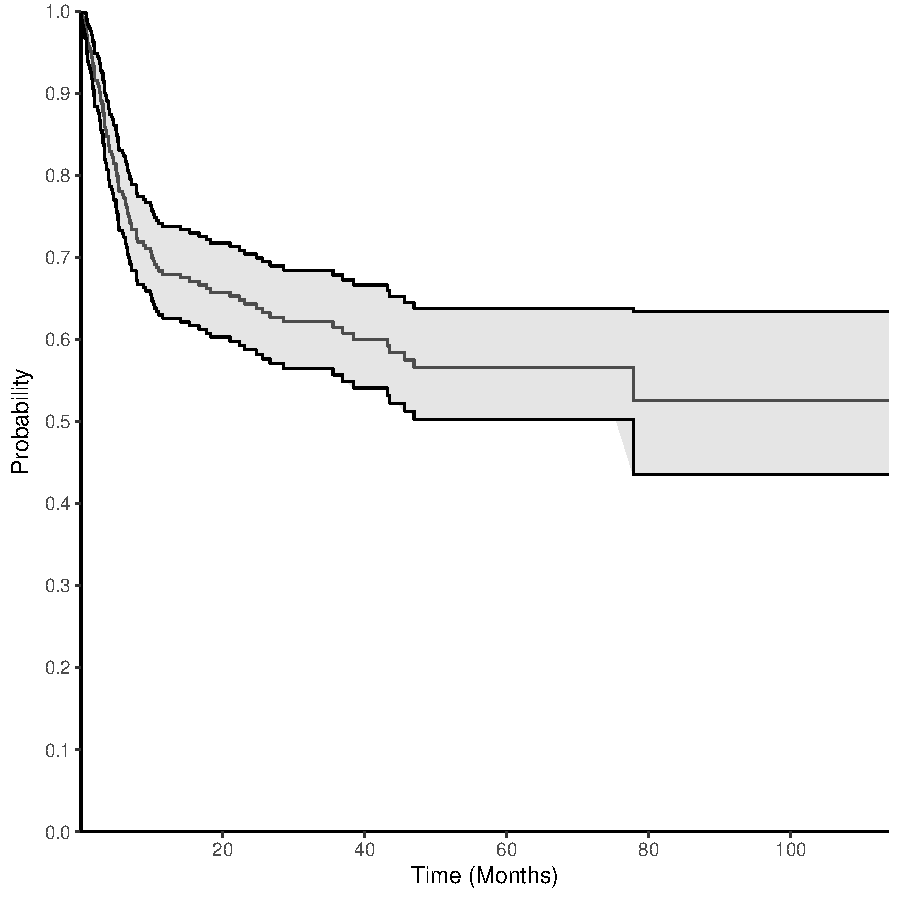
\includegraphics{Rapport-fig1}
\end{center}
\caption{KM Overall survival}
\label{fig1}
\end{figure}


\end{document}
